\section{Elimination of nondeterminism}

Every nondeterministic finite automaton can be transformed into an equivalent deterministic one. 
Consequently, every right-linear grammar has an equivalent non-ambiguous right-linear grammar. 
Therefore, any ambiguous regular expression can be transformed into a non-ambiguous one. 
The algorithm for converting a nondeterministic automaton into a deterministic one consists of two phases:
\begin{enumerate}
    \item Elimination of spontaneous moves: as these moves correspond to copy rules, it suffices to apply the algorithm for removing copy rules.
    \item Replacement of the non-deterministic multiple transitions by changing the automaton state set: this is the well-known subset construction.
\end{enumerate}
\begin{example}
    Consider the following example:
    \begin{figure}[H]
        \centering
        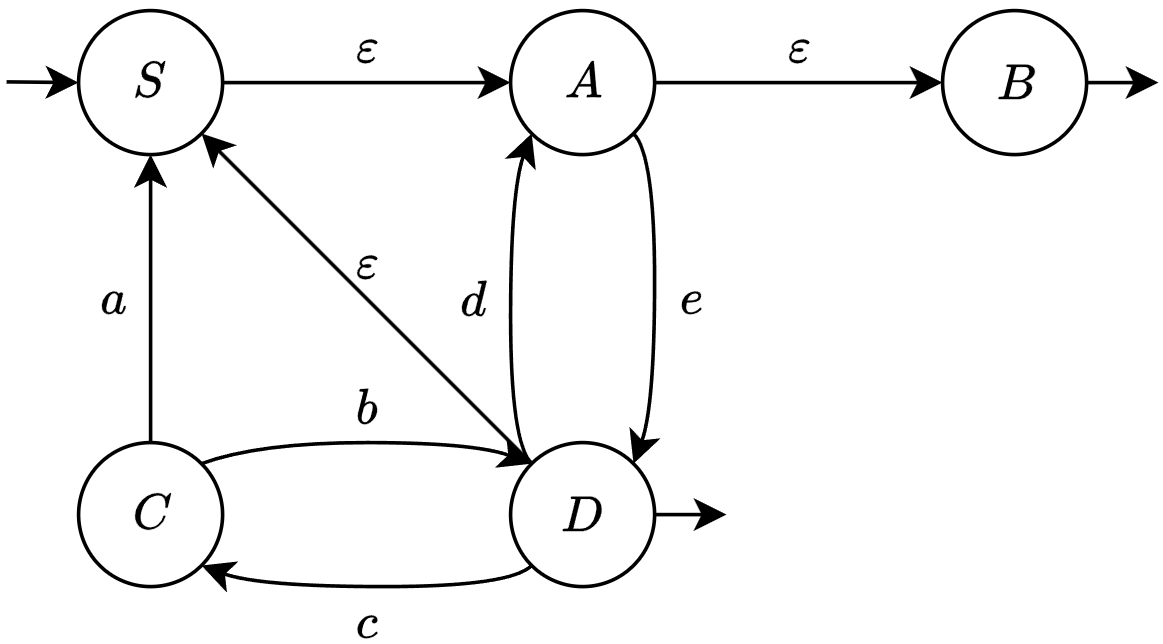
\includegraphics[width=0.5\linewidth]{images/oaut.png}
    \end{figure}
    After applying the algorithm, we obtain:
    \begin{figure}[H]
        \centering
        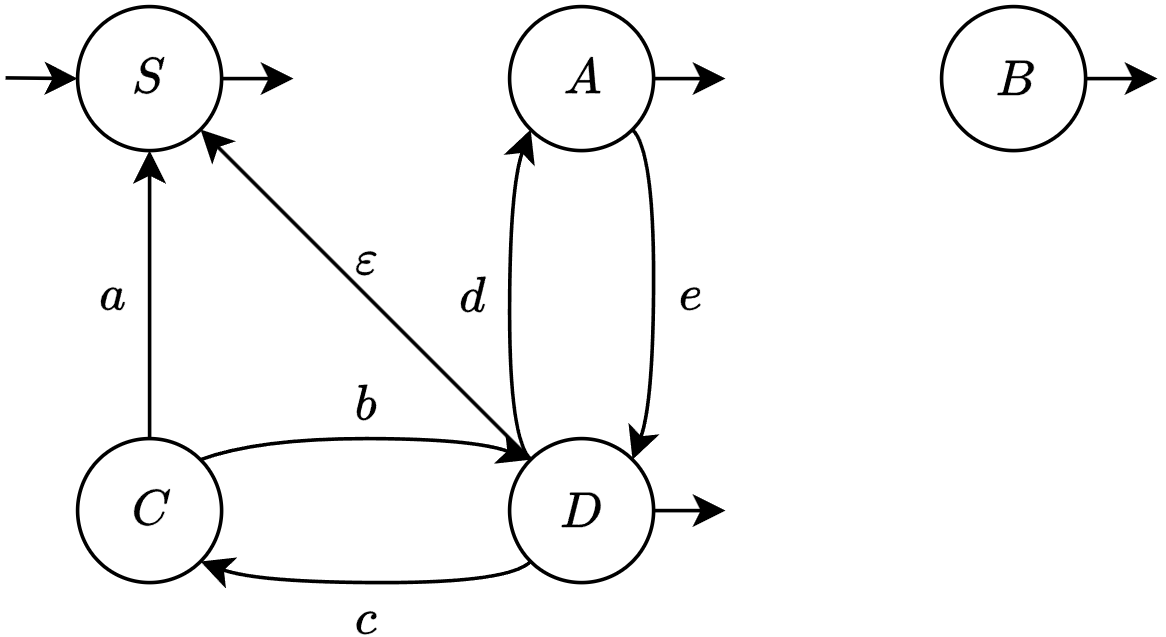
\includegraphics[width=0.5\linewidth]{images/faut.png}
    \end{figure}
    If, after eliminating all the $\varepsilon$-arcs, the automaton is still nondeterministic, proceed to the second phase.
\end{example}